\documentclass[aspectratio=169,10pt]{beamer}

\usepackage[utf8]{inputenc}
\usepackage[T1]{fontenc}
\usepackage{graphicx}
\usepackage{booktabs}
\usepackage{tabularx}
\usepackage{xcolor}
\usepackage{ragged2e}

\definecolor{navy}{HTML}{142B4A}
\definecolor{teal}{HTML}{148A8A}
\definecolor{coral}{HTML}{E5754E}
\definecolor{ink}{HTML}{233247}
\definecolor{muted}{HTML}{61748A}
\definecolor{pale}{HTML}{EEF3F7}

\setbeamercolor{normal text}{fg=ink,bg=white}
\setbeamercolor{structure}{fg=teal}
\setbeamercolor{frametitle}{fg=white,bg=navy}
\setbeamercolor{block title}{fg=white,bg=teal}
\setbeamercolor{block body}{fg=ink,bg=pale}
\setbeamercolor{alerted text}{fg=coral}
\setbeamertemplate{navigation symbols}{}
\setbeamertemplate{itemize item}{\color{teal}\scriptsize$\blacktriangleright$}
\setbeamertemplate{itemize subitem}{\color{coral}\tiny$\bullet$}
\setbeamertemplate{footline}{%
  \leavevmode\hbox{%
  \begin{beamercolorbox}[wd=.83\paperwidth,ht=2.6ex,dp=1.1ex,leftskip=1.2em]{author in head/foot}%
    \color{muted}\scriptsize CyED3 | Integrative Task 2 | Universidad Icesi
  \end{beamercolorbox}%
  \begin{beamercolorbox}[wd=.17\paperwidth,ht=2.6ex,dp=1.1ex,rightskip=1.2em plus1fil]{date in head/foot}%
    \color{muted}\scriptsize\insertframenumber/\inserttotalframenumber
  \end{beamercolorbox}}%
}
\setbeamertemplate{frametitle}{%
  \nointerlineskip
  \begin{beamercolorbox}[wd=\paperwidth,ht=3.5ex,dp=1.3ex,leftskip=1.1em]{frametitle}%
    \usebeamerfont{frametitle}\insertframetitle
  \end{beamercolorbox}
}
\graphicspath{{../outputs/figures/}}

\title{Sentiment Classification on Reddit}
\subtitle{GoEmotions | Dense, recurrent and Transformer models}
\author{Nicolas Mejia | Daniel Barragan | Jacobo Rodriguez}
\institute{Computability and Data Structures III | Universidad Icesi}
\date{November 2026}

\begin{document}

% 1
{\setbeamercolor{background canvas}{bg=navy}\setbeamertemplate{footline}{}
\begin{frame}[plain]
    \begin{minipage}[c][0.88\paperheight][c]{0.82\paperwidth}
      {\color{teal}\large INTEGRATIVE TASK 2}\par\vspace{0.45cm}
      {\color{white}\LARGE\bfseries Sentiment Classification\par}
      {\color{white}\LARGE\bfseries on Reddit\par}\vspace{0.35cm}
      {\color{white!80}\large GoEmotions | Dense | RNN | LSTM | DistilBERT}\par\vspace{1.1cm}
      {\color{white}\normalsize Nicolas Mejia | Daniel Barragan | Jacobo Rodriguez}\par
      {\color{white!70}\small Universidad Icesi | CyED3 | November 2026}
    \end{minipage}
\end{frame}}

% 2
\begin{frame}{Question and experimental setup}
\begin{columns}[T,onlytextwidth]
  \column{.54\textwidth}
    \begin{block}{Task}
      Predict whether a Reddit comment expresses \textbf{positive} or \textbf{negative} sentiment.
    \end{block}
    \vspace{0.25cm}
    \large\textbf{Research question}\par
    \normalsize Do sequence memory and self-attention improve sentiment classification over a fixed-vector model?
  \column{.42\textwidth}
    \begin{itemize}
      \item 1,000 balanced comments
      \item 800 train / 200 held-out test
      \item Same test comments for all models
      \item 5 seeds for baseline, Dense, RNN and LSTM; 3 for DistilBERT
      \item Accuracy, positive-class F1, macro F1 and Cohen's $\kappa$
    \end{itemize}
\end{columns}
\vfill
{\color{muted}\scriptsize The test split is not used to select hyperparameters.}
\end{frame}

% 3
\begin{frame}{From 54,263 comments to a balanced sample}
\begin{columns}[T,onlytextwidth]
  \column{.58\textwidth}
    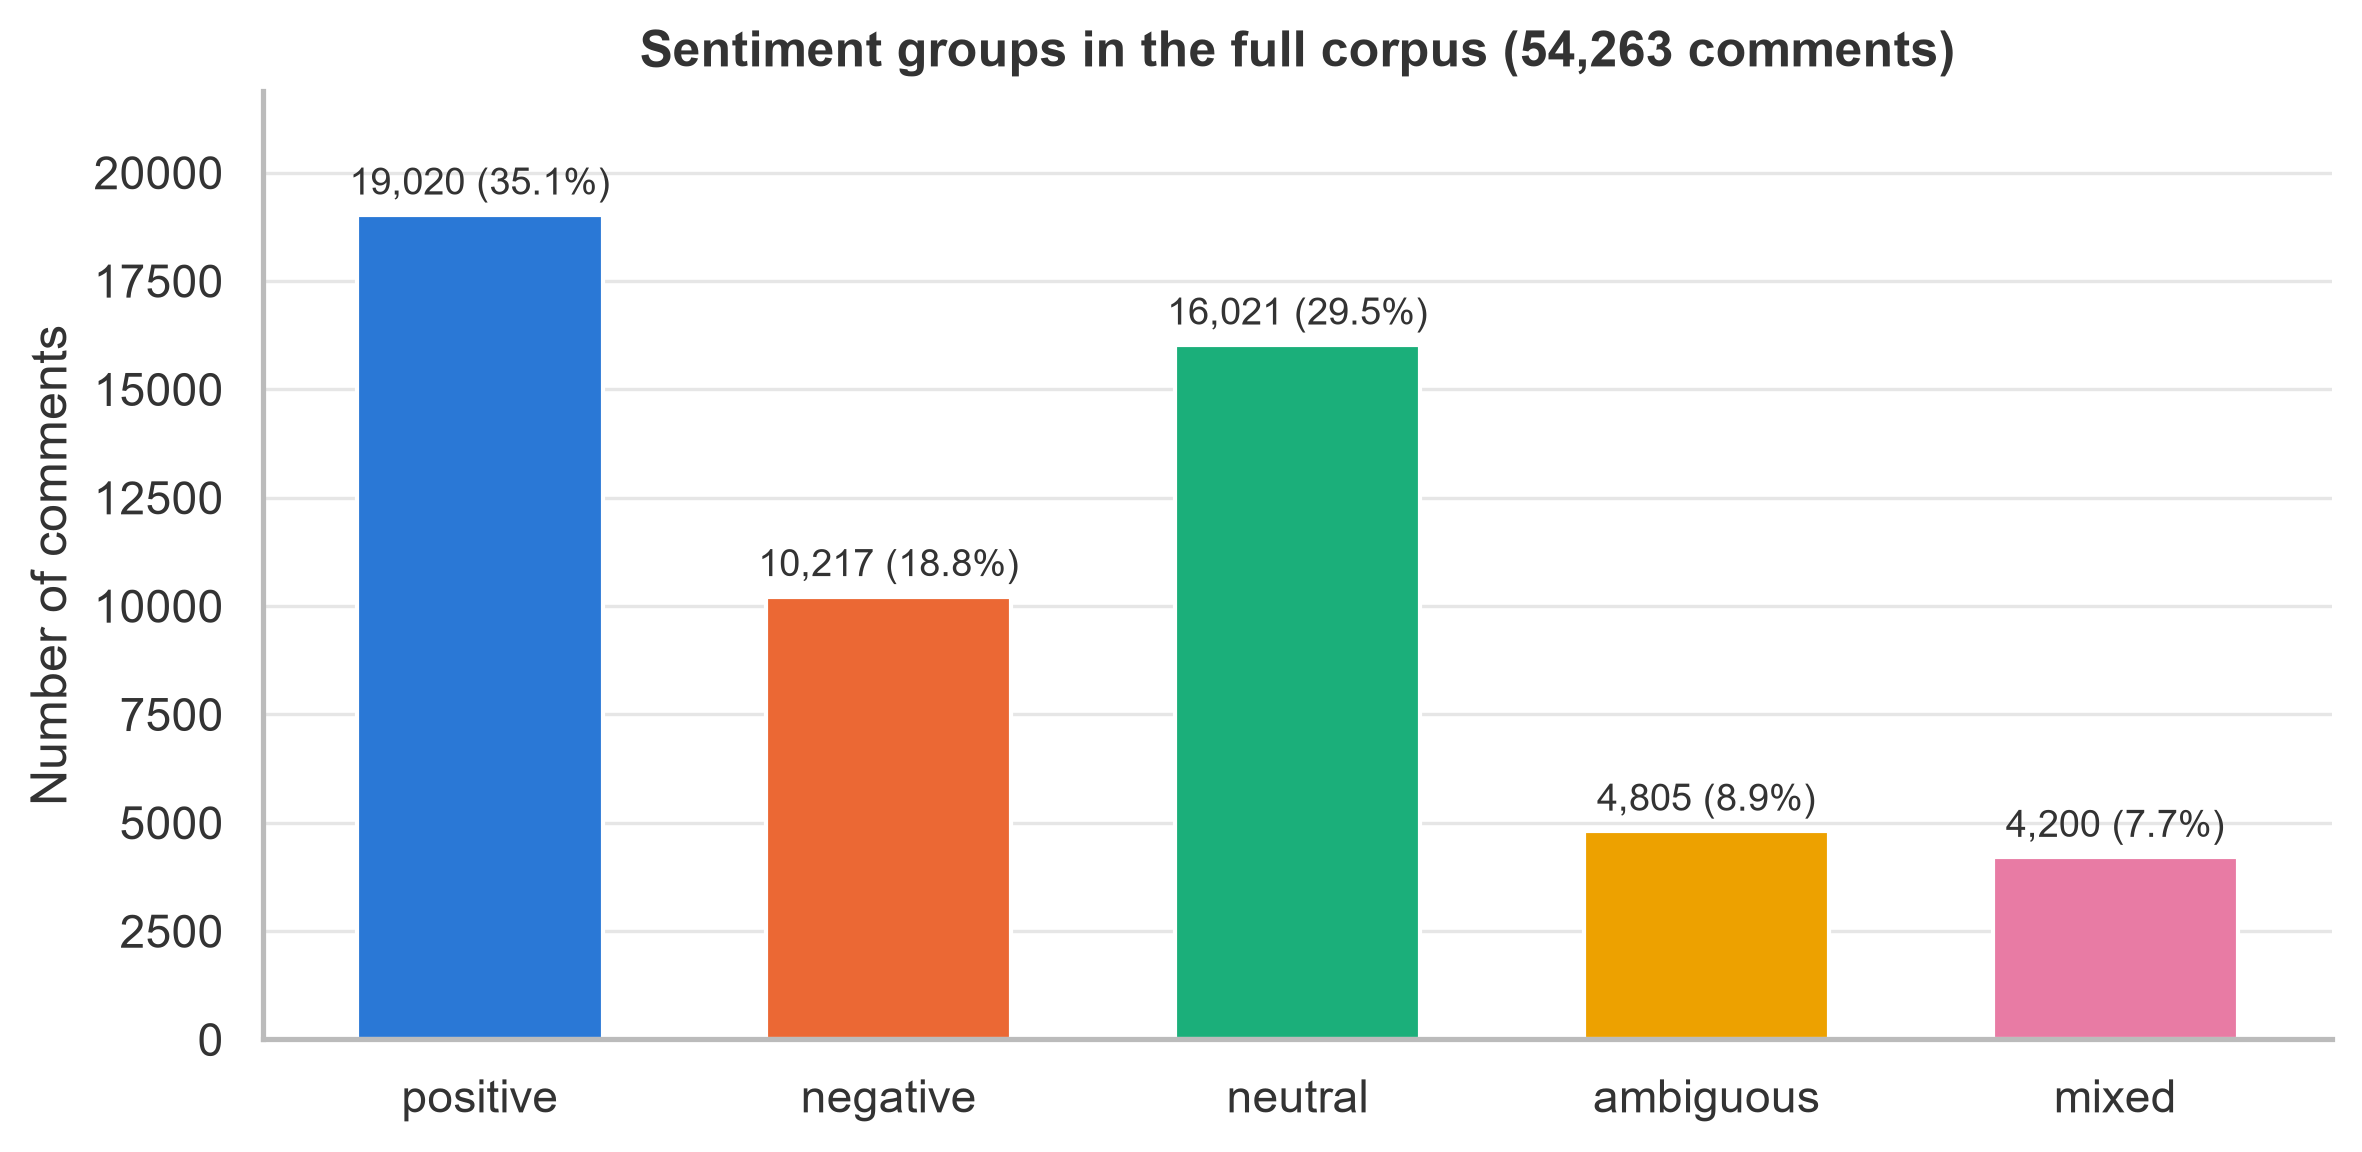
\includegraphics[width=\linewidth,height=.48\textheight,keepaspectratio]{eda_sentiment_groups.png}
    \par\vspace{0.08cm}
    {\centering\color{muted}\scriptsize Official emotion-to-sentiment mapping across the full corpus\par}
  \column{.38\textwidth}
    \begin{enumerate}
      \item Assign positive, negative, ambiguous, neutral or mixed using the official mapping.
      \item Keep only positive/negative comments; remove duplicate and conflicting text.
      \item Sample 500 per class with seed 42.
      \item Stratify into 800 train and 200 test comments.
    \end{enumerate}
    \begin{block}{Quality checks}
      1,000 unique; balanced train/test; no ID overlap
    \end{block}
\end{columns}
\vfill
{\color{muted}\scriptsize GoEmotions: Demszky et al. (2020).}
\end{frame}

% 4
\begin{frame}{Preprocessing preserves sentiment cues}
\begin{columns}[T,onlytextwidth]
  \column{.51\textwidth}
    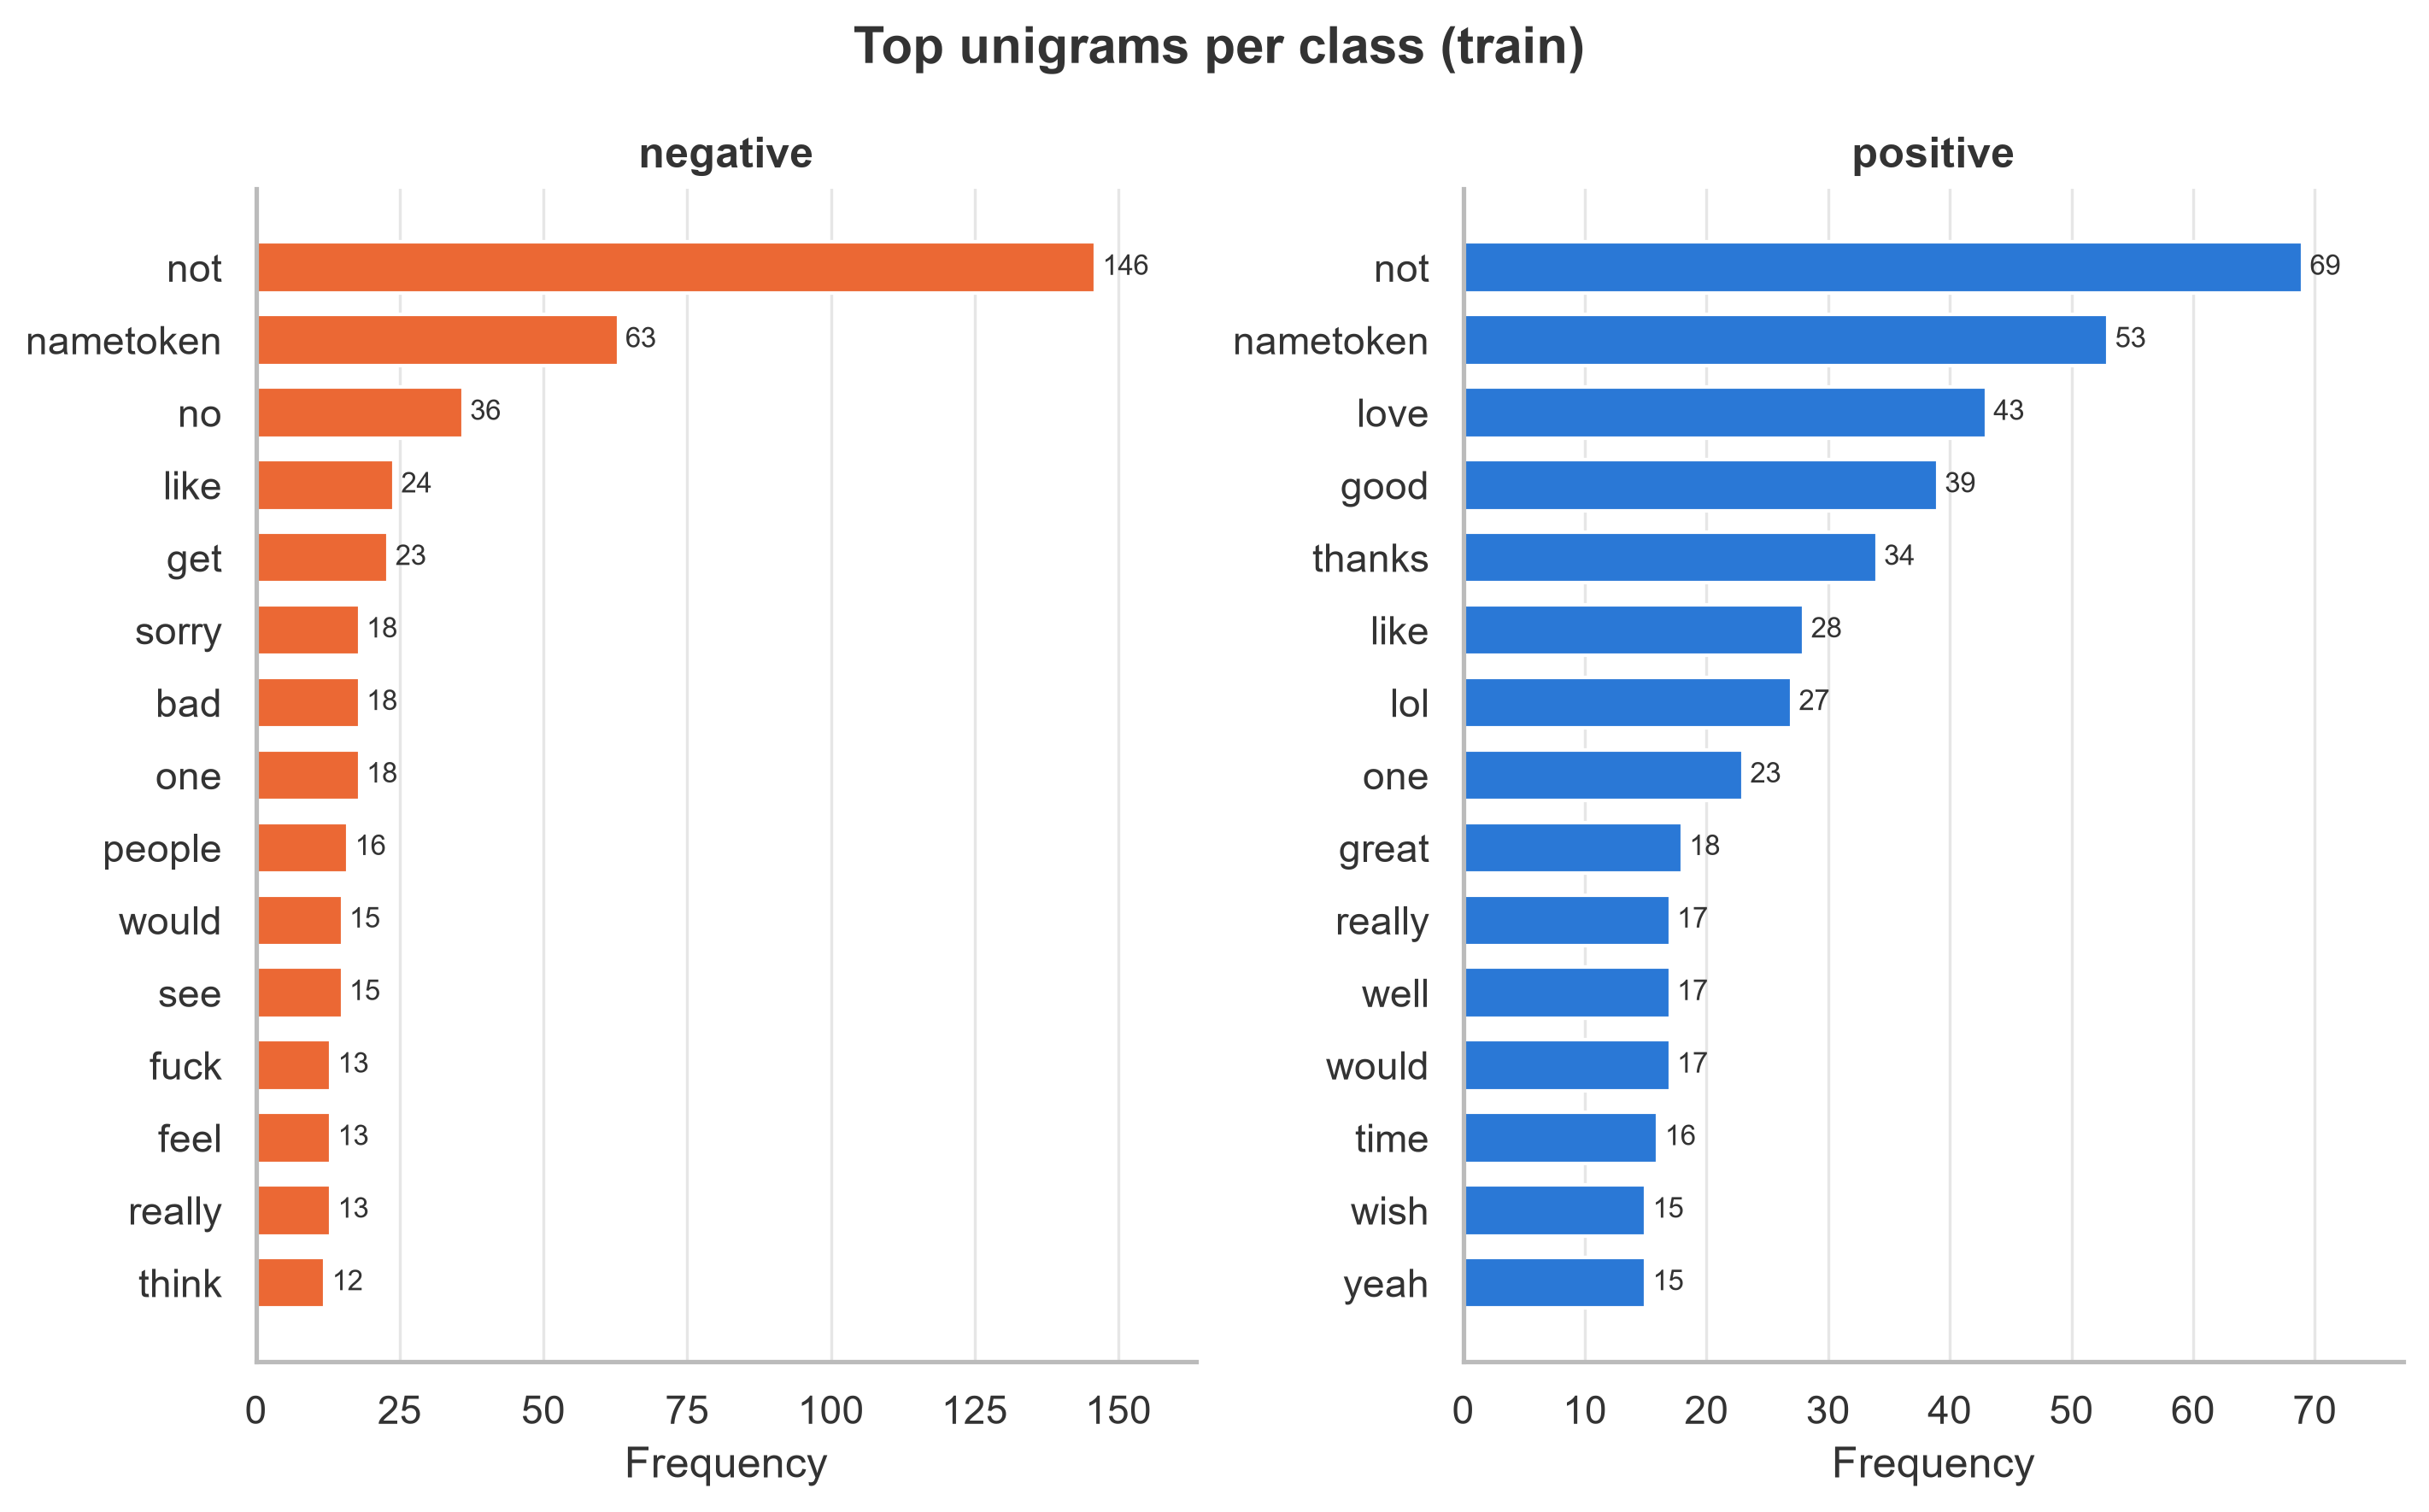
\includegraphics[width=\linewidth,height=.57\textheight,keepaspectratio]{eda_top_unigrams.png}
    \centering{\color{muted}\scriptsize Frequent cleaned tokens in the training split}
  \column{.45\textwidth}
    \begin{itemize}
      \item Normalize case, names, religion markers, URLs and punctuation.
      \item Convert emoji to text; tokenize and remove English stopwords.
      \item Keep negations such as \textit{not}, \textit{no} and \textit{never}.
      \item Keras models: vocabulary learned on train; sequences capped at 30 tokens.
      \item DistilBERT: raw text and pretrained subword tokenizer; max length 64.
    \end{itemize}
\end{columns}
\vfill
\begin{alertblock}{Why keep negation?}
  A rule that removes \textit{not} can turn ``not happy' into ``happy.' Negation appears in 32.6\% of negative and 16.8\% of positive comments.
\end{alertblock}
\end{frame}

% 5
\begin{frame}{Four model families, two input paths}
\small
\begin{columns}[T,onlytextwidth]
  \column{.235\textwidth}
    {\color{teal}\bfseries Dummy}\par\vspace{0.12cm}
    Samples from class frequency.\par\vspace{0.12cm}
    \color{muted}Baseline; does not read text.
  \column{.235\textwidth}
    {\color{teal}\bfseries Dense}\par\vspace{0.12cm}
    Mean word embeddings $\rightarrow$ dense layers.\par\vspace{0.12cm}
    \color{muted}No token order or recurrent state.
  \column{.235\textwidth}
    {\color{teal}\bfseries SimpleRNN / LSTM}\par\vspace{0.12cm}
    Read tokens sequentially; update a hidden state. LSTM gates a cell memory.\par\vspace{0.12cm}
    \color{muted}Bounded learned state.
  \column{.235\textwidth}
    {\color{coral}\bfseries DistilBERT}\par\vspace{0.12cm}
    Pretrained subword encoder; self-attention connects tokens across the context.\par\vspace{0.12cm}
    \color{muted}Parallel, bounded context.
\end{columns}
\vspace{0.55cm}
\begin{block}{Fair comparison}
  Dense, RNN and LSTM share train-only vectorization and embeddings. DistilBERT uses its own tokenizer on raw text.
\end{block}
\vfill
{\color{muted}\scriptsize Elman (1990); Hochreiter \& Schmidhuber (1997); Vaswani et al. (2017); Sanh et al. (2019).}
\end{frame}

% 6
\begin{frame}{Hyperparameter selection keeps test data held out}
\begin{columns}[T,onlytextwidth]
  \column{.32\textwidth}
    \begin{block}{Keras models}
      680 fit / 120 validation\par
      48 settings per architecture\par
      Select by validation macro F1\par
      Refit on 800 train comments\par
      Evaluate seeds 42--46
    \end{block}
  \column{.32\textwidth}
    \begin{block}{DistilBERT}
      Same 680/120 split\par
      2e-5 vs 5e-5 learning rate\par
      3 epochs; select checkpoint by validation macro F1\par
      Refit seeds 42--44
    \end{block}
  \column{.32\textwidth}
    \begin{block}{Final test}
      One fixed set of 200 comments\par
      Train and test metrics for all five models\par
      Mean $\pm$ sample SD across seeds\par
      Compare latency on CPU
    \end{block}
\end{columns}
\vfill
{\centering\color{muted}\scriptsize Validation selected $2\times10^{-5}$ for DistilBERT (macro F1 0.8667 vs 0.8666).\par}
\end{frame}

% 7
\begin{frame}{DistilBERT leads mean test macro F1}
\begin{columns}[T,onlytextwidth]
  \column{.69\textwidth}
    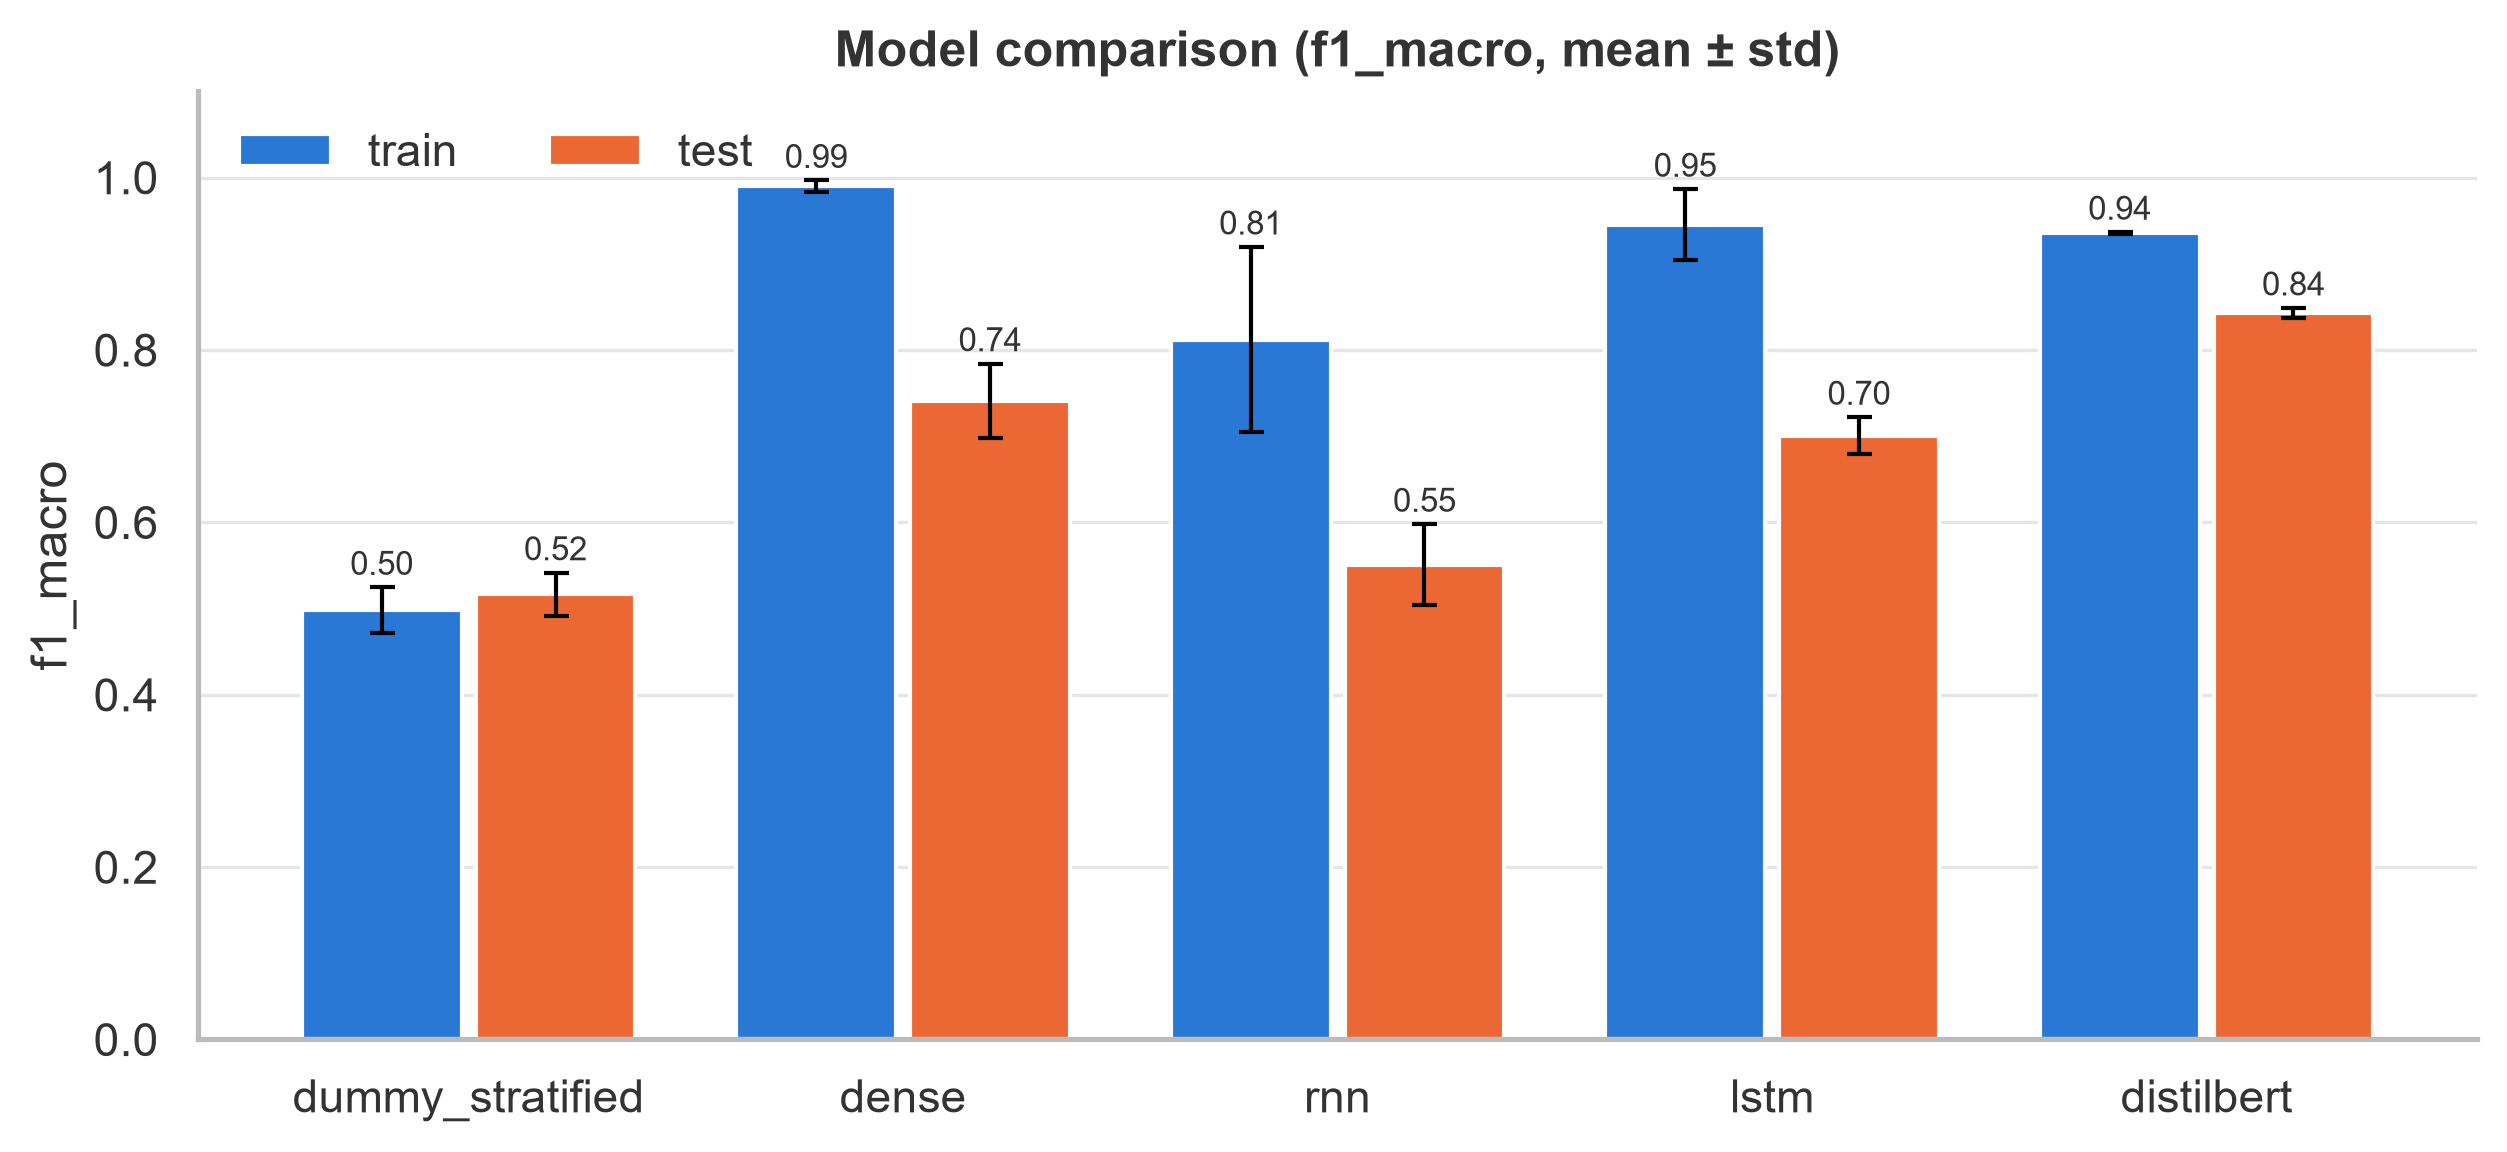
\includegraphics[width=\linewidth,height=.64\textheight,keepaspectratio]{comparison.png}
  \column{.27\textwidth}
    {\color{coral}\Huge\bfseries 0.843}\par
    {\color{ink}\normalsize DistilBERT test macro F1}\par\vspace{0.35cm}
    \textbf{0.843 $\pm$ 0.006} accuracy\par
    \textbf{0.687 $\pm$ 0.012} Cohen's $\kappa$\par\vspace{0.35cm}
    Dense: 0.741 $\pm$ 0.043 macro F1\par
    \vspace{0.25cm}
    {\color{muted}\scriptsize DistilBERT: 3 seeds; others: 5. Same 200 test comments. Descriptive comparison, not a significance test.}
\end{columns}
\end{frame}

% 8
\begin{frame}{Attention views are diagnostic, not causal}
\begin{columns}[T,onlytextwidth]
  \column{.48\textwidth}
    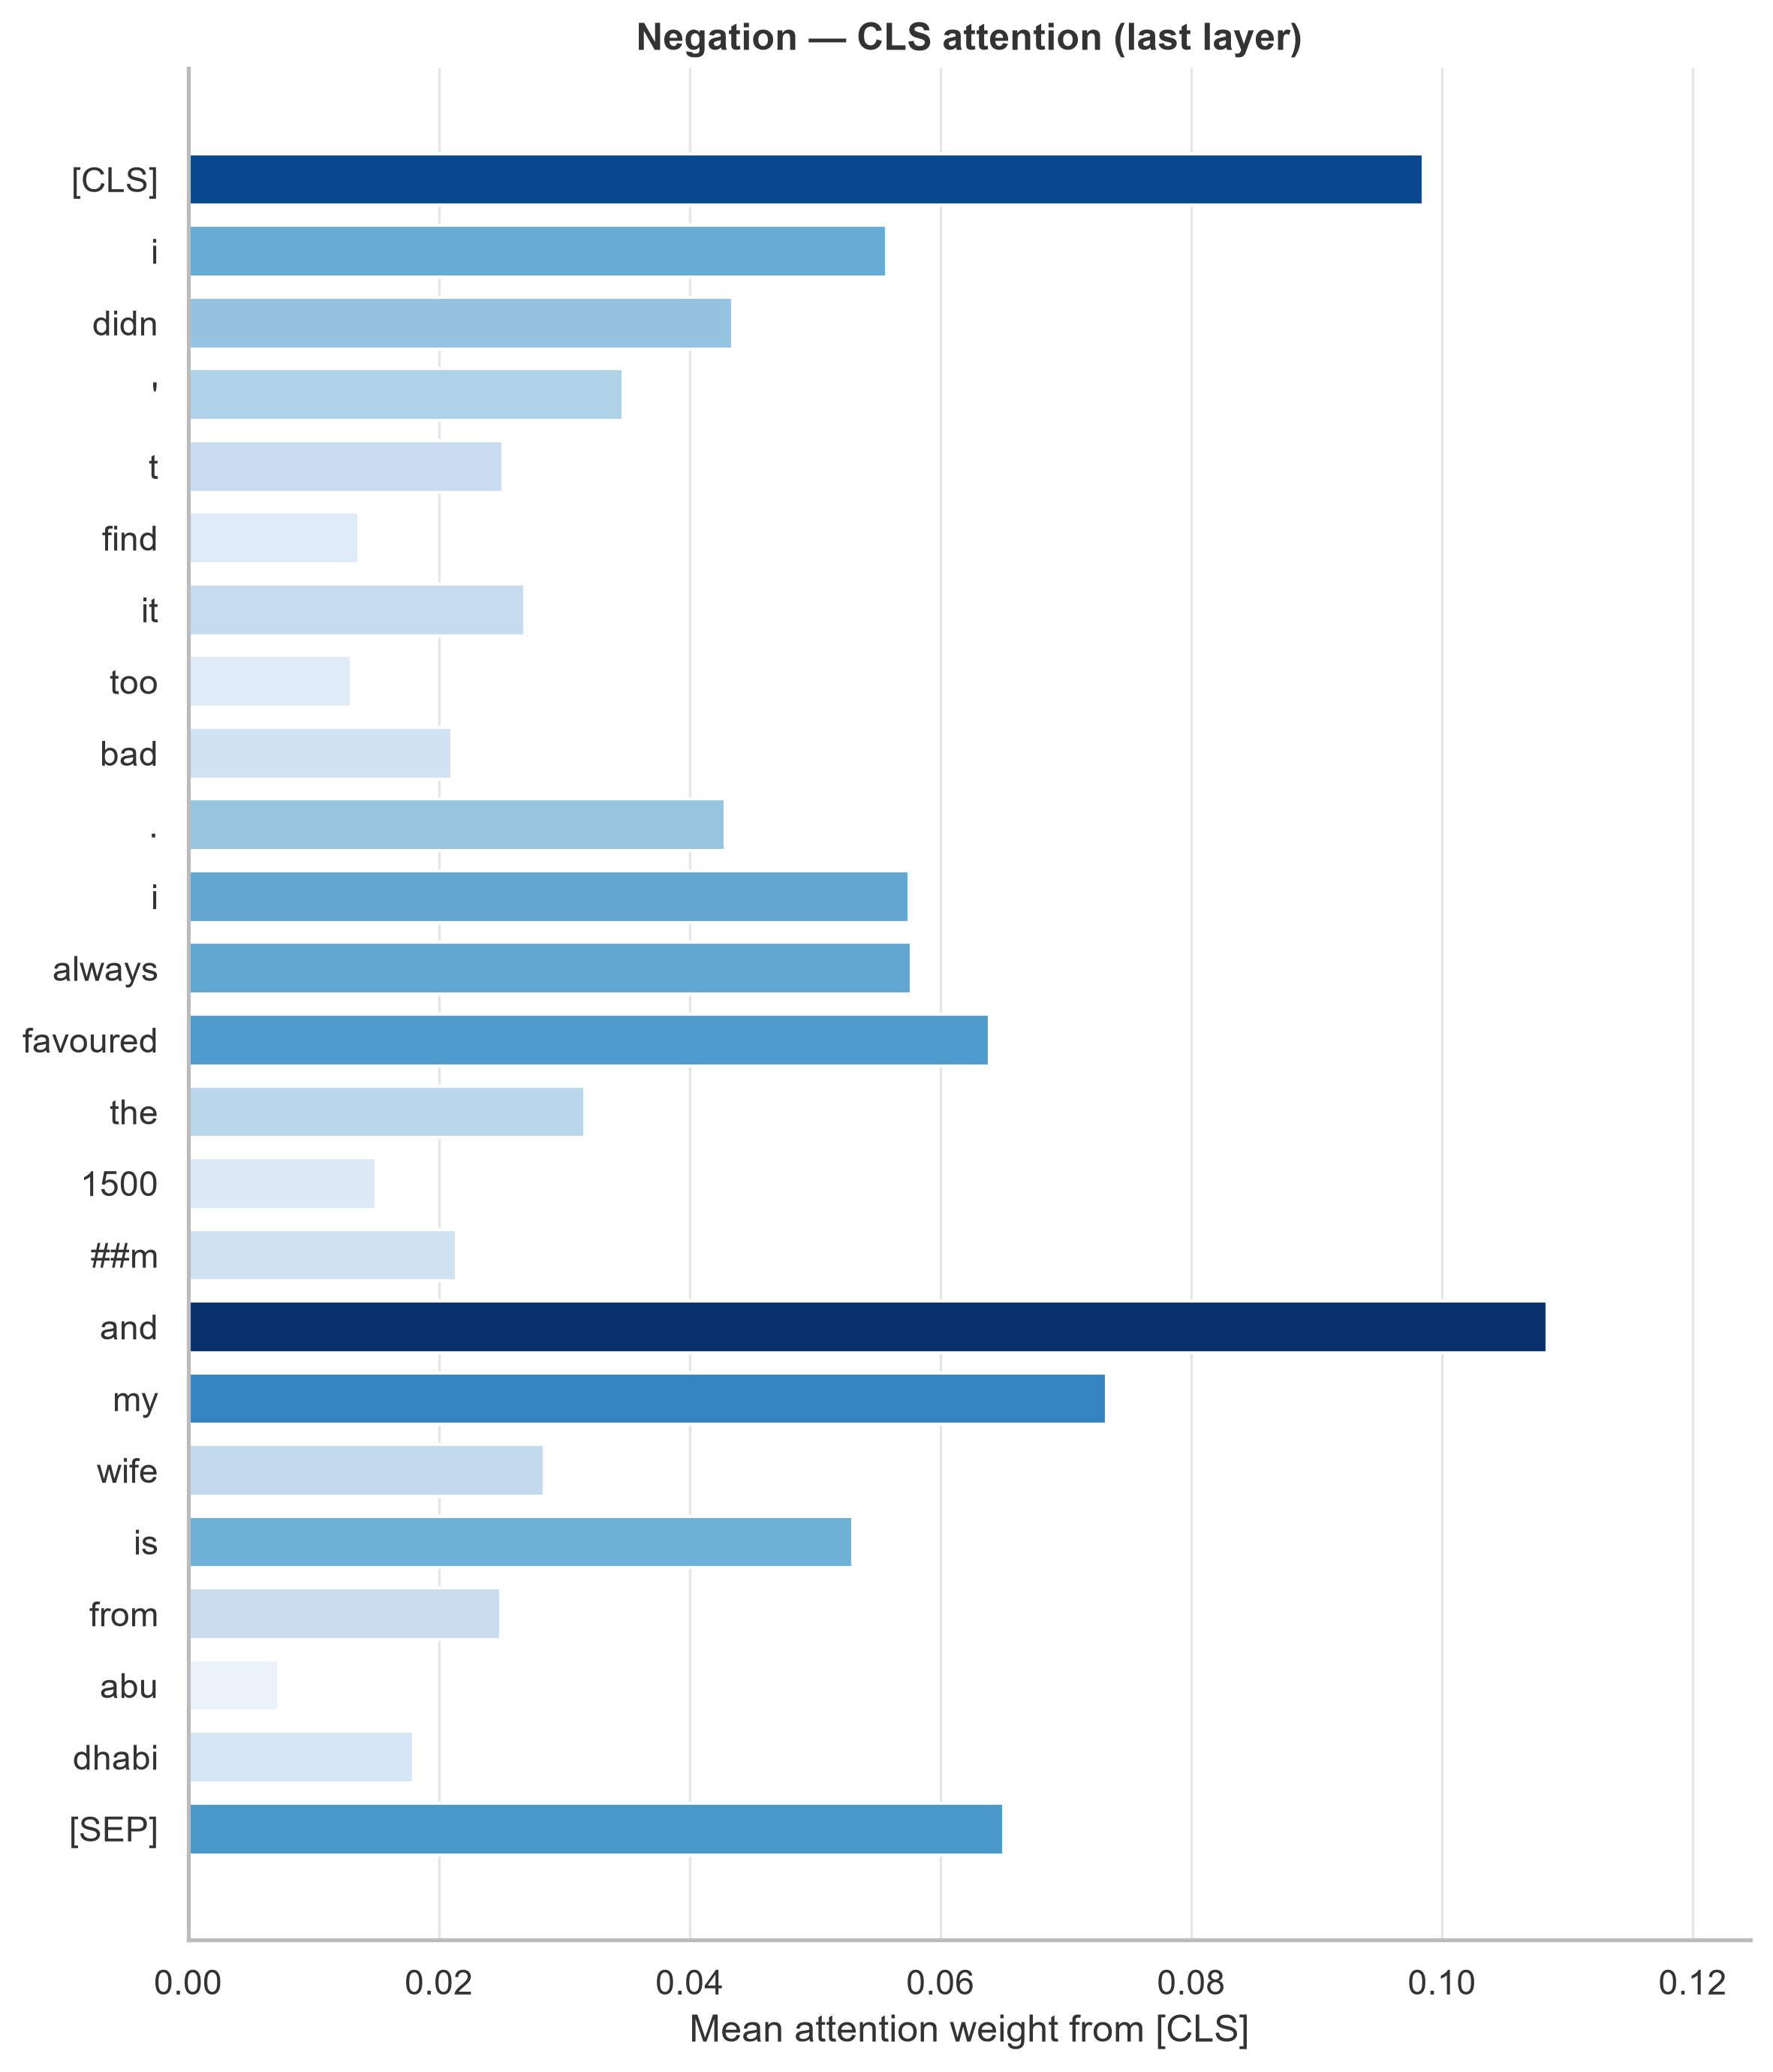
\includegraphics[width=\linewidth,height=.44\textheight,keepaspectratio]{attention_cls_negation.png}\par\vspace{0.08cm}
    {\centering\small Negation\par}
  \column{.48\textwidth}
    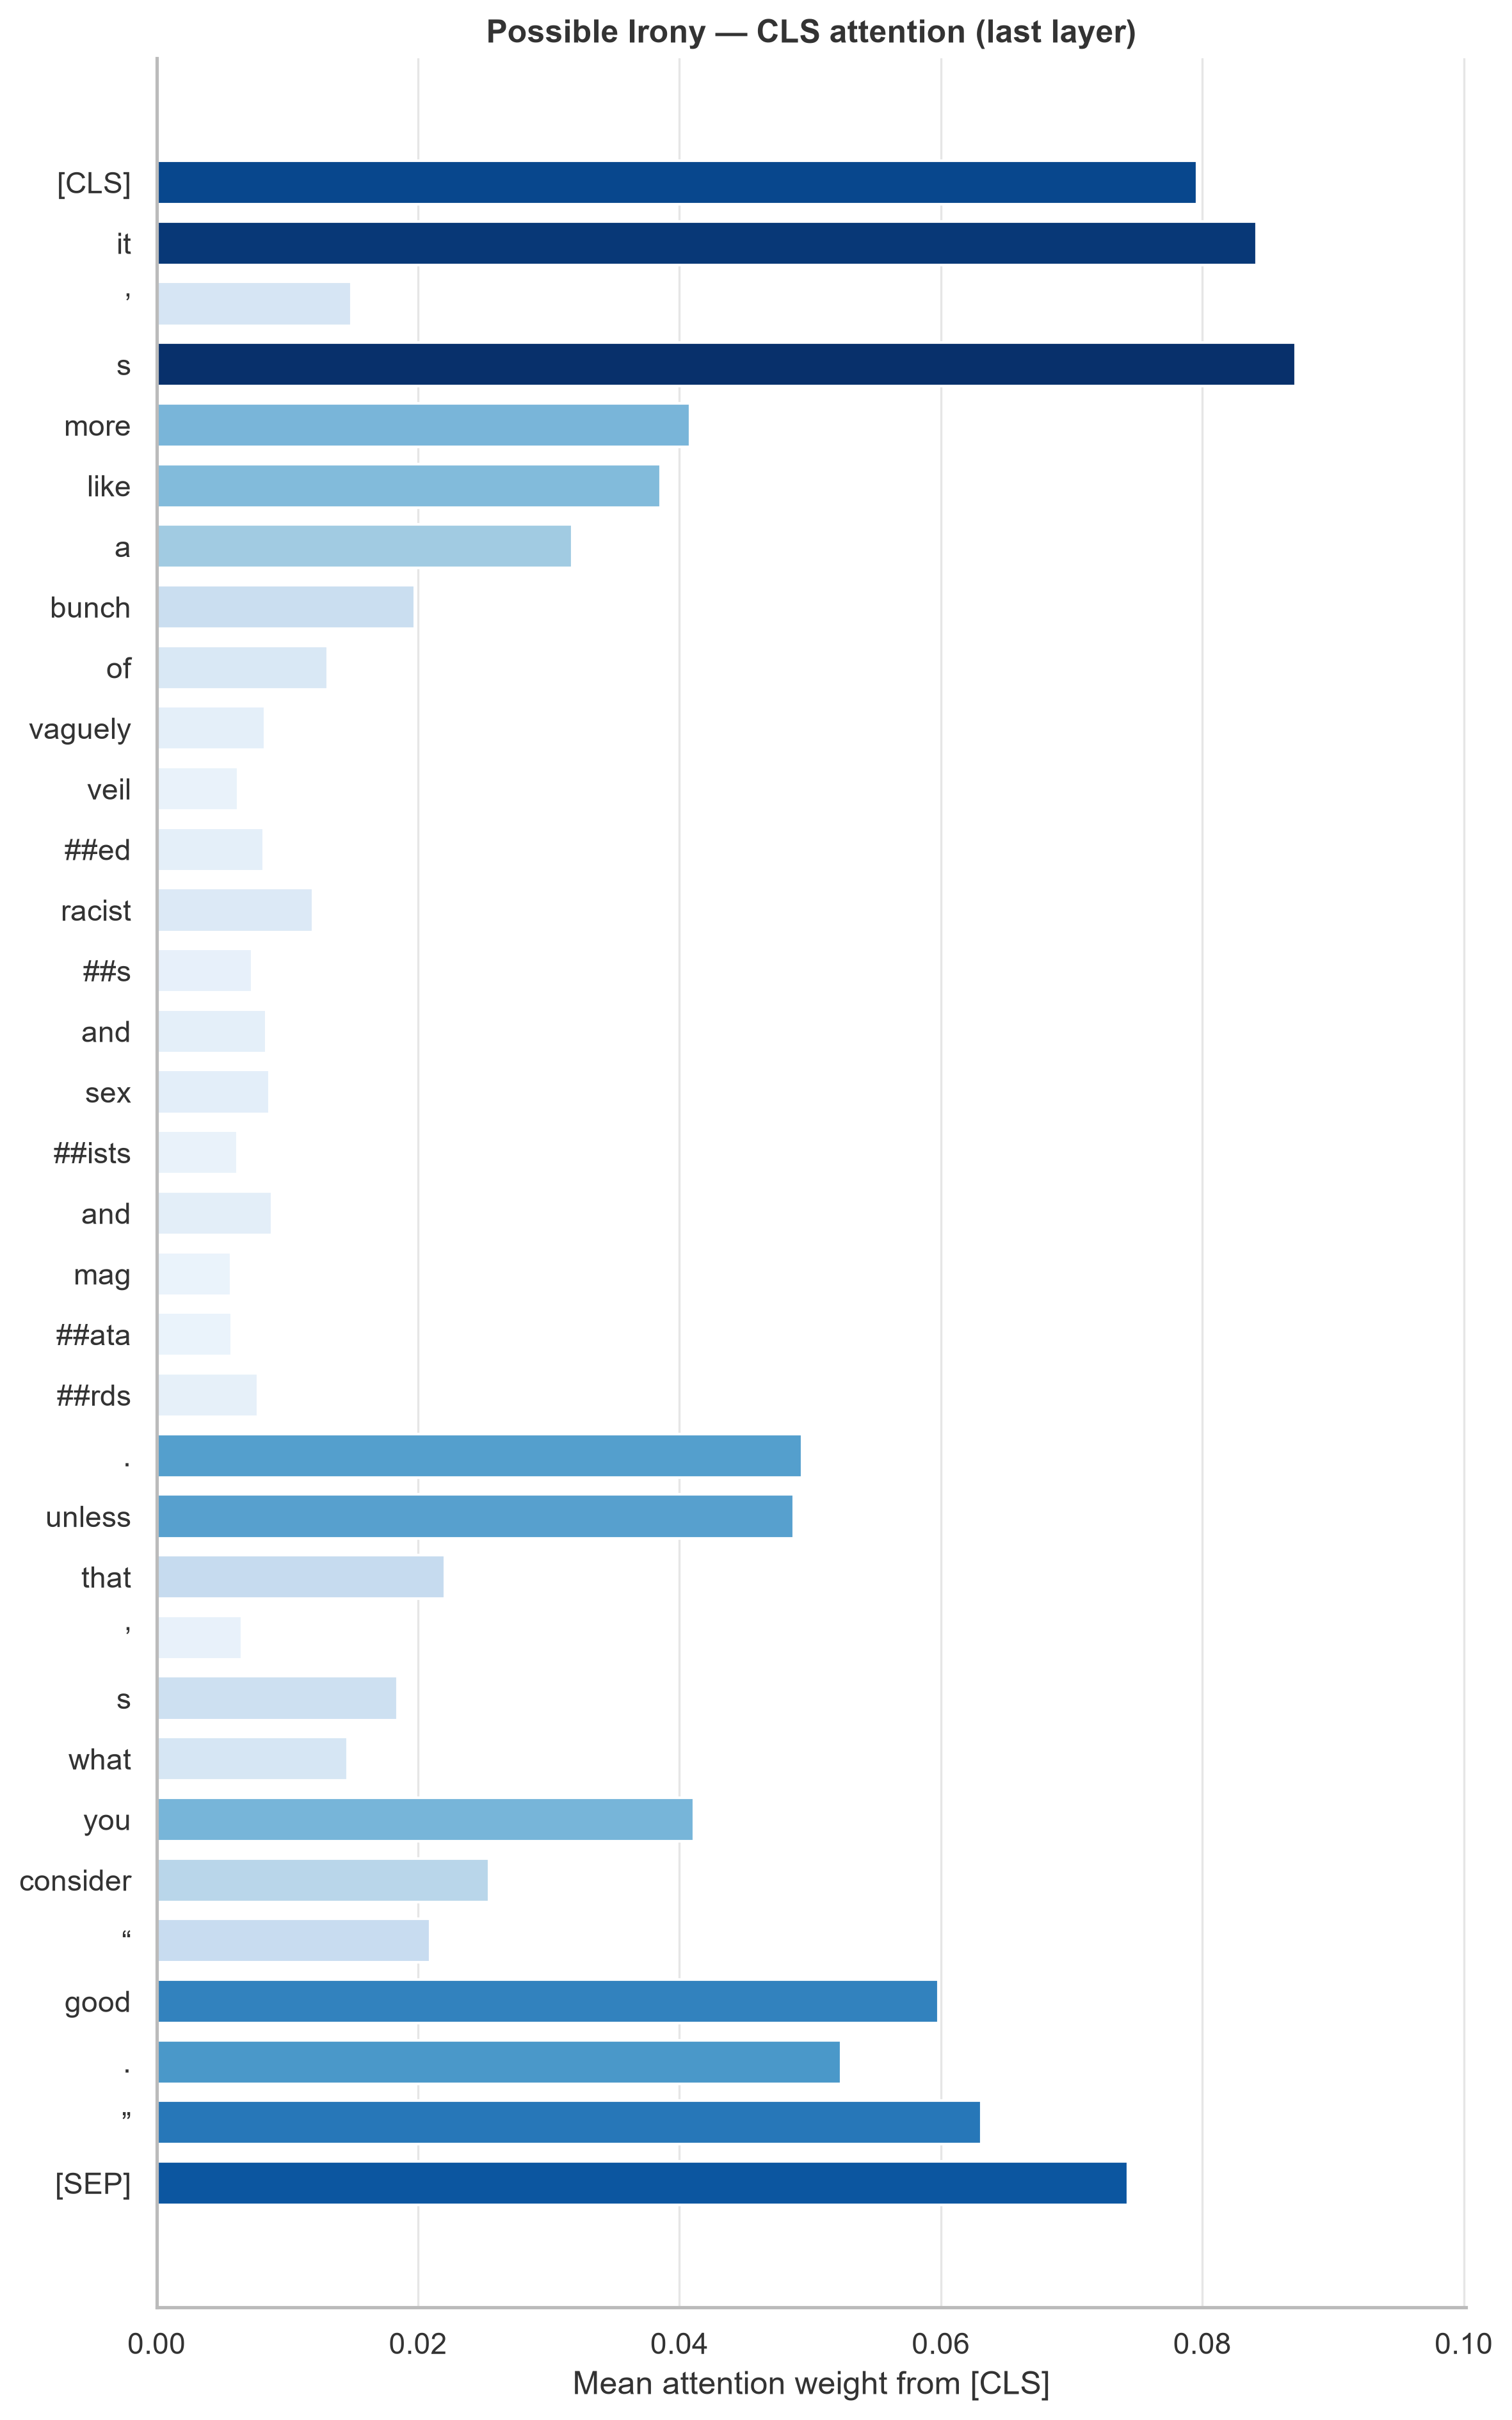
\includegraphics[width=\linewidth,height=.44\textheight,keepaspectratio]{attention_cls_possible_irony.png}\par\vspace{0.08cm}
    {\centering\small Possible irony\par}
\end{columns}
\vspace{0.08cm}
\begin{columns}[T,onlytextwidth]
  \column{.48\textwidth}
    Dense exposes pooled token effects but loses word order. RNN and LSTM keep order in hidden states that are harder to inspect. LSTM had fewer false positives than SimpleRNN (23 vs. 61), but more false negatives (34 vs. 21) on the selected checkpoints.
  \column{.48\textwidth}
    DistilBERT exposes final-layer [CLS] attention weights for inspection. They show attention allocation, but do not prove why a prediction occurred.
\end{columns}
\end{frame}

% 9
\begin{frame}{Training cost, inference and computability}
\begin{columns}[T,onlytextwidth]
  \column{.55\textwidth}
    \textbf{Measured CPU time}\par\vspace{0.1cm}
    {\scriptsize
    \begin{tabular}{@{}lrr@{}}
      \toprule
      Model & Final fit (s) & Infer./1k (s) \\
      \midrule
      Dummy & $<0.001$ & 0.0005 \\
      Dense & $0.86\pm0.06$ & 0.184 \\
      SimpleRNN & $1.30\pm0.11$ & 0.185 \\
      LSTM & $1.51\pm0.12$ & 0.221 \\
      DistilBERT & $644.9\pm424.1$ & 47.193 \\
      \bottomrule
    \end{tabular}\par
    }\vspace{0.12cm}
    {\color{muted}\scriptsize Final-fit mean $\pm$ SD across five seeds, three for DistilBERT; excludes tuning search. Inference covers 1,000 tokenized comments.}\par
    \small Parameters: Dense 76.8K; RNN 82.0K; LSTM 163.9K; DistilBERT 66.96M.
  \column{.4\textwidth}
    \begin{itemize}
      \item Dense averages token vectors in $O(Td)$ time.
      \item RNN and LSTM use sequential $O(T(dh+h^2))$ updates; LSTM gates add work.
      \item DistilBERT attention grows as $O(T^2d)$ per layer, with a 64-token limit.
      \item Turing-completeness results use idealized assumptions. These fixed, finite-precision models always terminate.
    \end{itemize}
\end{columns}
\vfill
{\color{muted}\scriptsize Inference excludes cleaning/tokenization; fit time excludes tuning search. CPU-only measurements. Sources: Siegelmann \& Sontag (1995); Graves et al. (2014); Pérez et al. (2021).}
\end{frame}

% 10
\begin{frame}{Conclusion and next steps}
\begin{columns}[T,onlytextwidth]
  \column{.54\textwidth}
    \begin{block}{What the results support}
      DistilBERT has the highest mean test macro F1 on this split. Dense offers a much faster CPU inference path. All neural models show a train/test gap.
    \end{block}
    \vspace{0.2cm}
    \begin{itemize}
      \item Test on a larger, independently sampled set and another comment source.
      \item Re-measure inference on deployment hardware, including GPU.
      \item Target negation, irony and emoji in error analysis.
    \end{itemize}
  \column{.4\textwidth}
    \textbf{10-minute presentation}\par\vspace{0.2cm}
    Nicolas | data and EDA | ~3 min\par
    Daniel | architectures and tuning | ~3 min\par
    Jacobo | Transformer, comparison and computability | ~4 min\par\vspace{0.3cm}
    \begin{alertblock}{Discussion}
      When is a 0.10 macro-F1 gain worth the inference cost?
    \end{alertblock}
\end{columns}
\vfill
{\color{muted}\scriptsize Selected sources: Demszky et al. (2020); Hochreiter \& Schmidhuber (1997); Sanh et al. (2019); Vaswani et al. (2017); Siegelmann \& Sontag (1995); Pérez et al. (2021).}
\end{frame}

\end{document}
